% Two-page, two-column report (IEEE-conference look, as in the BTP report used as format reference).
% IEEEtran.cls was not available in the build sandbox, so the look is reproduced with article+twocolumn.
% On Overleaf you may instead use \documentclass[conference]{IEEEtran}; the content below is compatible.
% All numbers come from numbers.tex / results_table.tex, generated by make_report_assets.py from the saved CSV files.
\documentclass[10pt,twocolumn]{article}
\usepackage[a4paper,top=0.6in,bottom=0.6in,left=0.58in,right=0.58in,columnsep=0.2in]{geometry}
\usepackage[T1]{fontenc}
\usepackage{mathptmx}
\usepackage{amsmath,amssymb}
\usepackage{graphicx,booktabs,url}
\usepackage{microtype}
\usepackage[font=footnotesize,labelsep=period,justification=justified,singlelinecheck=false]{caption}
\captionsetup[figure]{name={Fig.}}
\captionsetup[table]{name={TABLE},labelsep=newline,justification=centering,font={footnotesize,sc},position=top}
\renewcommand{\thetable}{\Roman{table}}
\usepackage{titlesec}
\renewcommand{\thesection}{\Roman{section}}
\renewcommand{\thesubsection}{\Alph{subsection}}
\titleformat{\section}[block]{\centering\footnotesize\scshape}{\thesection.}{0.5em}{}
\titleformat{\subsection}[block]{\normalfont\small\itshape}{\thesubsection.}{0.5em}{}
\titlespacing*{\section}{0pt}{5pt}{2pt}
\titlespacing*{\subsection}{0pt}{3pt}{1pt}
\usepackage{enumitem}\setlist{nosep,leftmargin=1.2em}
\usepackage[hidelinks]{hyperref}
\newcommand{\NTrainSteps}{300\,000}
\newcommand{\NBestStep}{275}
\newcommand{\NWallTime}{139}
\newcommand{\NValBest}{-612}
\newcommand{\NValPassive}{-829}
\newcommand{\NAccHoLo}{22}
\newcommand{\NAccHoHi}{43}
\newcommand{\NAccRandLo}{22}
\newcommand{\NAccRandHi}{26}
\newcommand{\NDtlRandLo}{22}
\newcommand{\NDtlRandHi}{25}
\newcommand{\NDtlBumpOne}{+2.6}
\newcommand{\NSatMax}{0.0}
\newcommand{\NPeakForceMax}{1046}
\newcommand{\NEarlyTerm}{0}
\newcommand{\NSkyAccC}{8.5}
\newcommand{\NSkyDtlC}{+0.2}
\newcommand{\NTermAccP}{1.34}
\newcommand{\NTermAccN}{0.64}
\newcommand{\NTermDefP}{0.21}
\newcommand{\NTermDefN}{0.26}
\newcommand{\NTermTyreP}{0.31}
\newcommand{\NTermTyreN}{0.48}
\newcommand{\NTermTotP}{1.86}
\newcommand{\NTermTotN}{1.38}
\newcommand{\NClDP}{1.4}
\newcommand{\NClDN}{4.3}
\newcommand{\NAllPaired}{all}
\newcommand{\NNEpisodes}{113}
\newcommand{\NNSeeds}{3}
\newcommand{\NValBestAll}{-612, -594, -602}
\newcommand{\NValDipAll}{-5925}
\newcommand{\NSeedAccRandLo}{22}
\newcommand{\NSeedAccRandHi}{26}
\newcommand{\NSeedDtlRandLo}{20}
\newcommand{\NSeedDtlRandHi}{29}

\newcommand{\repourl}{https://github.com/TODO-replace-with-team-repo}% <-- REPLACE with the real GitHub URL
\setlength{\parindent}{1em}\setlength{\parskip}{0pt}
\setlength{\textfloatsep}{5pt plus 2pt minus 2pt}\setlength{\floatsep}{4pt plus 2pt minus 2pt}\setlength{\intextsep}{4pt plus 2pt minus 2pt}
\setlength{\abovedisplayskip}{2pt}\setlength{\belowdisplayskip}{2pt}
\pagestyle{empty}
\AtBeginDocument{\fontsize{9.7}{11}\selectfont}

\begin{document}
\twocolumn[{%
\begin{center}
{\fontsize{17}{19}\selectfont RL-Based Active Suspension Control\\[1pt] Using a Quarter-Car Simulation}\\[5pt]
{\footnotesize
\begin{tabular}{@{}c@{\hspace{30pt}}c@{}}
\textbf{Darshan Prajapati} (B23CH1032) & \textbf{Sunny Kumar} (B23ME1073)\\
b23ch1032@iitj.ac.in & b23me1073@iitj.ac.in
\end{tabular}\\[2pt]
Indian Institute of Technology Jodhpur --- AI Course Mini Project (Assignment 2)\\[2pt]
\textbf{GitHub:} \url{\repourl}}
\end{center}\vspace{2pt}}]

\noindent{\footnotesize\textbf{\textit{Abstract}---Passive car suspensions trade ride comfort against road holding. We cast active quarter-car suspension as continuous-control RL: six sensor observations, one bounded force action, a quadratic reward, trained with PPO. On held-out roads PPO cuts body acceleration \NAccHoLo--\NAccHoHi\% versus passive but worsens tyre-load variation.}}

\vspace{2pt}\noindent{\footnotesize\textbf{\textit{Index Terms}---reinforcement learning, PPO, active suspension, quarter-car model, ride comfort, road holding.}}

\section{Problem and Motivation}
A passive suspension (spring $k_s$, damper $c_s$) trades \emph{ride comfort} (low body acceleration) against \emph{road holding} (small dynamic tyre-load variation) and bounded \emph{suspension travel}. An active suspension adds a force actuator, but must act on an unknown random road with limited sensing and a saturating actuator. We pose this as a partially observed MDP and learn a policy with Proximal Policy Optimization (PPO)~\cite{ppo}. The simulator, environment and evaluation code were written for this project; only NumPy, Gymnasium~\cite{gym} and Stable-Baselines3~\cite{sb3} are used as libraries, and no existing RL repository was copied.

\section{Quarter-Car Dynamics}
With $z$ up and displacements from static equilibrium (gravity cancels), body $z_s$, wheel $z_u$, road $z_r$, actuator force $u$:
\begin{align}
m_s\ddot z_s &= -k_s(z_s-z_u)-c_s(\dot z_s-\dot z_u)+u,\\
m_u\ddot z_u &= k_s(z_s-z_u)+c_s(\dot z_s-\dot z_u)-k_t(z_u-z_r)-u.
\end{align}
Parameters (plausible round values, \emph{not} identified from a real car): $m_s{=}290$ kg, $m_u{=}59$ kg, $k_s{=}16$ kN/m, $c_s{=}1$ kN\,s/m, $k_t{=}190$ kN/m (body mode 1.18 Hz, wheel hop 9.40 Hz, $\zeta{\approx}0.23$). Integration: fixed-step RK4, 1 ms, force held constant over each 10 ms control step; episode 10 s (1000 steps). Roads are $C^1$ profiles at constant speed, $z_r(t){=}z(vt)$: flat, raised-cosine bump, and ISO~8608-style random roads~\cite{iso8608} (classes A--E, $G_d(n){=}G_d(n_0)(n/n_0)^{-2}$, 100 random-phase cosines). Assumptions: linear spring/damper/tyre, no bump stops, no tyre lift-off (tyre-load ratio $1{+}F_t/((m_s{+}m_u)g)\le0$ is only \emph{flagged}), ideal actuator without lag.

\section{RL Formulation}
\subsection{State (observation) space $\mathcal S$}
$o_k\in\mathbb R^{6}$ (dimension 6; fixed normalisation, no clipping):
\[
o_k=\Big[\tfrac{\ddot z_s}{2},\ \tfrac{z_s-z_u}{0.05},\ \tfrac{\dot z_s-\dot z_u}{0.5},\ \tfrac{z_u-z_r}{0.01},\ \tfrac{\dot z_u}{0.5},\ a_{k-1}\Big].
\]
Road velocity and the upcoming road are \emph{not} observed, so the problem is partially observed.
\subsection{Action space $\mathcal A$}
Continuous $a_k\in[-1,1]$, force $u_k=\mathrm{clip}(a_k)\,u_{\max}$, $u_{\max}{=}1500$ N ($u{>}0$ pushes the body up and the wheel down).
\subsection{Reward $R$}
With overbars the mean over the 10 sub-steps of a control step, $d{=}z_s{-}z_u$, $F_t{=}k_t(z_u{-}z_r)$:
\begin{equation}
r_k=-\Big[w_a\tfrac{\overline{\ddot z_s^{2}}}{a_{\rm ref}^2}+w_d\tfrac{\overline{d^{2}}}{d_{\rm ref}^2}+w_t\tfrac{\overline{F_t^{2}}}{F_{\rm ref}^2}+w_u a_k^2+w_{\Delta}\big(\tfrac{a_k-a_{k-1}}{2}\big)^{2}\Big],
\end{equation}
$(w_a,w_d,w_t,w_u,w_\Delta){=}(1,0.3,0.3,0.05,0.05)$, $a_{\rm ref}{=}1$ m/s$^2$, $d_{\rm ref}{=}0.015$ m, $F_{\rm ref}{=}0.25(m_s{+}m_u)g{=}856$ N. The scales are the rounded RMS response of the passive car on ISO~C at 15 m/s, so each term is $O(1)$ and the weights express priority (comfort first). Safety-guard termination ($|d|{>}0.30$ m, $|z_u{-}z_r|{>}0.15$ m, non-finite state) costs 10 per remaining step; it never occurred (\NEarlyTerm\ of \NNEpisodes\ PPO evaluation episodes). Weights are a first choice, \emph{not} tuned.

\section{Environment and PPO Training}
The Gymnasium environment resamples road, speed and seed at each reset. \textbf{Training mixture:} flat (10--20 m/s); bump ($h{\in}[0.02,0.04]$ m, $L{\in}[1.5,3]$ m, 8--14 m/s); ISO B and C (10--20 m/s). PPO suits the bounded continuous force, the cheap simulator and needs stable updates (clipped objective). Stable-Baselines3 setup: MLP actor/critic $64{\times}64$ tanh; 4 envs $\times$ 1000-step rollouts; batch 500; 10 epochs; learning rate $3{\times}10^{-4}$; $\gamma{=}0.99$; GAE $\lambda{=}0.95$; clip 0.2; entropy coef.\ 0; seed 0; \NTrainSteps\ steps (\NWallTime~s, one CPU core). Only the reward is normalised (running statistics). Every 25k steps the policy is validated on six fixed seeds (90000--90005) of the training mixture; the best checkpoint (\NBestStep k steps) is kept. Evaluation seeds ($\ge$100000) are never used for training or selection.

\begin{figure}[t]\centering
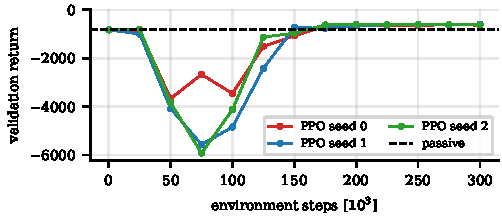
\includegraphics[width=\columnwidth]{fig_curve.pdf}
\caption{Validation return of PPO (mean$\pm$std, 6 seeds) vs passive on the same seeds (higher is better). Best checkpoint: \NValBest; passive: \NValPassive.}\label{fig:curve}
\end{figure}

\section{Baseline and Evaluation Protocol}
The \textbf{passive baseline} applies $u{\equiv}0$ on the identical vehicle; $c_s{=}1000$ N\,s/m gave the highest passive reward on ISO B/C in a sweep over 500--4000 (stiffer damping lowers tyre-load variation but raises acceleration). PPO (deterministic) and passive are run on the \emph{same} road, speed, reset seed and initial state (road height asserted identical). In Table~\ref{tab:res}: \textbf{T}=training distribution; \textbf{U}=unseen road class A or unseen initial offset (body +20 mm); \textbf{H}=held-out: taller/longer/faster bump ($h{=}0.055$ m, $L{=}3.5$ m, 16 m/s), ISO D at 10 m/s, and the `test' mixture (tall bump; ISO A at 22--28 m/s; ISO D at 8--12 m/s). Random roads use 20--30 seeds, deterministic scenarios 1. Metrics are physical (unweighted RMS acceleration, no ISO~2631 filter; deflection; RMS dynamic tyre load; contact-loss flag; actuator force); return is kept separate. A hand-designed skyhook law $u{=}-1500\,\dot z_s$~\cite{skyhook} (\emph{not RL}, untuned) serves only as a reference.

\begin{figure*}[t]\centering
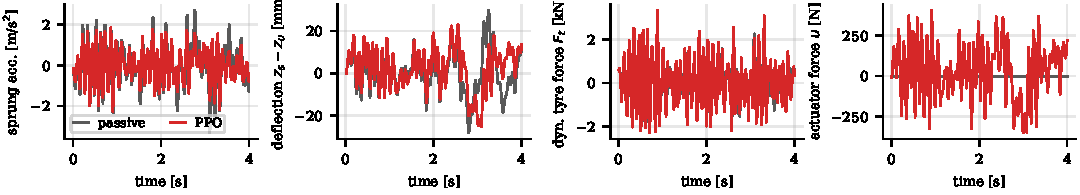
\includegraphics[width=\textwidth]{fig_time.pdf}
\caption{Passive vs PPO on an ISO-C road, 15 m/s (seed 100000, first 4 s): body acceleration, suspension deflection, dynamic tyre force, and PPO actuator force (passive: 0 N).}\label{fig:time}
\end{figure*}

\begin{table*}[t]\centering
\caption{PPO vs passive under matched conditions (means over $n$ episodes, seeds $\ge$100000)}\label{tab:res}
\scriptsize\setlength{\tabcolsep}{3.6pt}
\begin{tabular}{@{}lrrrrrrrrrr@{}}\toprule
 & & \multicolumn{2}{c}{RMS acc [m/s$^2$]} & \multicolumn{4}{c}{PPO change vs passive [\%] ($+$ = better)} & Skyhook & PPO & Contact-loss\\
\cmidrule(lr){3-4}\cmidrule(lr){5-8}
Scenario (set) & $n$ & passive & PPO & RMS acc & peak acc & RMS defl & RMS tyre & RMS acc [\%] & RMS $u$ [N] & steps [\%] pass./PPO\\\midrule
bump 10 m/s (T) & 1 & 0.386 & 0.197 & +49.1 & +37.0 & +3.3 & +2.6 & +15.8 & 68 & 0.0/0.0 \\
ISO B 15 m/s (T) & 20 & 0.575 & 0.437 & +24.0 & +23.9 & -18.2 & -22.8 & +8.5 & 104 & 0.0/0.0 \\
ISO C 15 m/s (T) & 20 & 1.149 & 0.877 & +23.6 & +21.8 & -12.3 & -23.6 & +8.5 & 194 & 0.0/0.1 \\
ISO A 15 m/s (U) & 20 & 0.287 & 0.218 & +24.0 & +24.1 & -36.3 & -22.2 & +8.5 & 61 & 0.0/0.0 \\
flat, +20 mm start (U) & 1 & 0.131 & 0.035 & +73.6 & +70.2 & -46.7 & +72.3 & +37.6 & 52 & 0.0/0.0 \\
tall bump 16 m/s (H) & 1 & 0.541 & 0.309 & +43.0 & +33.7 & +1.2 & -5.9 & +10.3 & 88 & 0.0/0.0 \\
ISO D 10 m/s (H) & 20 & 1.861 & 1.447 & +22.2 & +21.0 & -8.6 & -24.6 & +8.3 & 296 & 1.4/4.3 \\
test mixture (H) & 30 & 0.925 & 0.683 & +26.2 & +25.7 & -8.9 & -22.1 & +9.4 & 152 & 0.5/1.4\\
\bottomrule\end{tabular}
\end{table*}

\section{Results}
Fig.~\ref{fig:curve}: validation return passes the passive level after $\approx$175k steps and is noisy before. \textbf{Comfort:} PPO lowers RMS and peak body acceleration in every scenario: \NAccRandLo--\NAccRandHi\% on random roads (\NAllPaired\ paired seeds better), \NAccHoLo--\NAccHoHi\% on the three held-out cases, 49\% on the in-distribution bump; the untuned skyhook reference gives about \NSkyAccC\%. \textbf{Trade-offs:} on random roads RMS tyre load is \NDtlRandLo--\NDtlRandHi\% \emph{worse} than passive, deflection is worse in most scenarios, and the contact-loss flag on ISO~D rises from \NClDP\% to \NClDN\% of steps; skyhook leaves tyre load unchanged (\NSkyDtlC\% on ISO~C). On the 10 m/s bump tyre load changes by \NDtlBumpOne\%. \textbf{Effort:} moderate (RMS 52--296 N, peak $\le$\NPeakForceMax\ N, saturation \NSatMax\%).

\begin{figure}[t]\centering
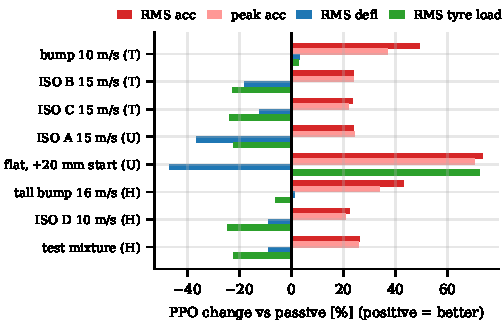
\includegraphics[width=\columnwidth]{fig_bars.pdf}
\caption{Change of PPO relative to passive per scenario and metric (from Table~\ref{tab:res} data; positive = better, negative = degradation). Comfort gains come with negative tyre-load and deflection bars on most scenarios.}\label{fig:bars}
\end{figure}

\section{Discussion and Conclusion}
Mean per-step reward terms on ISO~C (passive$\to$PPO) are: acceleration \NTermAccP$\to$\NTermAccN, deflection \NTermDefP$\to$\NTermDefN, tyre force \NTermTyreP$\to$\NTermTyreN, total \NTermTotP$\to$\NTermTotN. PPO thus optimises the stated objective, buying a large comfort gain with higher tyre-force and travel terms (comfort weight 1.0 vs 0.3); a larger $w_t$ should shift this balance (not tested). \emph{Limitations:} one training seed (evaluation spread reflects road variability only); a 1M-step run gave no better validation return; untuned weights; unweighted acceleration; linear tyre; ideal actuator; unvalidated parameters; hidden road velocity. A PPO policy trained on a road mixture thus generalised to unseen and held-out roads for comfort, at a clear road-holding cost; we do not claim superiority over passive suspension. \textbf{Reproducibility:} code, trained model, result CSVs and the commands to regenerate every table and figure of this report are in the repository (\texttt{README.md}); numbers here are generated from the saved CSV files.

\begingroup\footnotesize\setlength{\itemsep}{0pt}
\begin{thebibliography}{9}\setlength{\itemsep}{0pt}\setlength{\parsep}{0pt}
\bibitem{ppo} J.~Schulman, F.~Wolski, P.~Dhariwal, A.~Radford, O.~Klimov, ``Proximal policy optimization algorithms,'' arXiv:1707.06347, 2017.
\bibitem{sb3} A.~Raffin \emph{et al.}, ``Stable-Baselines3: Reliable reinforcement learning implementations,'' \emph{J. Mach. Learn. Res.}, vol.~22, no.~268, pp.~1--8, 2021.
\bibitem{gym} M.~Towers \emph{et al.}, ``Gymnasium: A standard interface for reinforcement learning environments,'' arXiv:2407.17032, 2024.
\bibitem{iso8608} ISO 8608:2016, \emph{Mechanical vibration---Road surface profiles---Reporting of measured data}.
\bibitem{skyhook} D.~Karnopp, M.~J.~Crosby, R.~A.~Harwood, ``Vibration control using semi-active force generators,'' \emph{J. Eng. Ind.}, vol.~96, no.~2, pp.~619--626, 1974.
\end{thebibliography}\endgroup
% Optional (team decision, check course policy on AI assistance): add an acknowledgment of any AI-assisted code/report drafting.
\end{document}
